%==============================================================================
% Figure: F4 Root System Projection
% Purpose: 2D projection of F4 root system showing 48 roots
% Chapter: Ch03 - Exceptional Lie Groups
% Type: Mathematical
%==============================================================================

\begin{figure}[htbp]
  \centering
  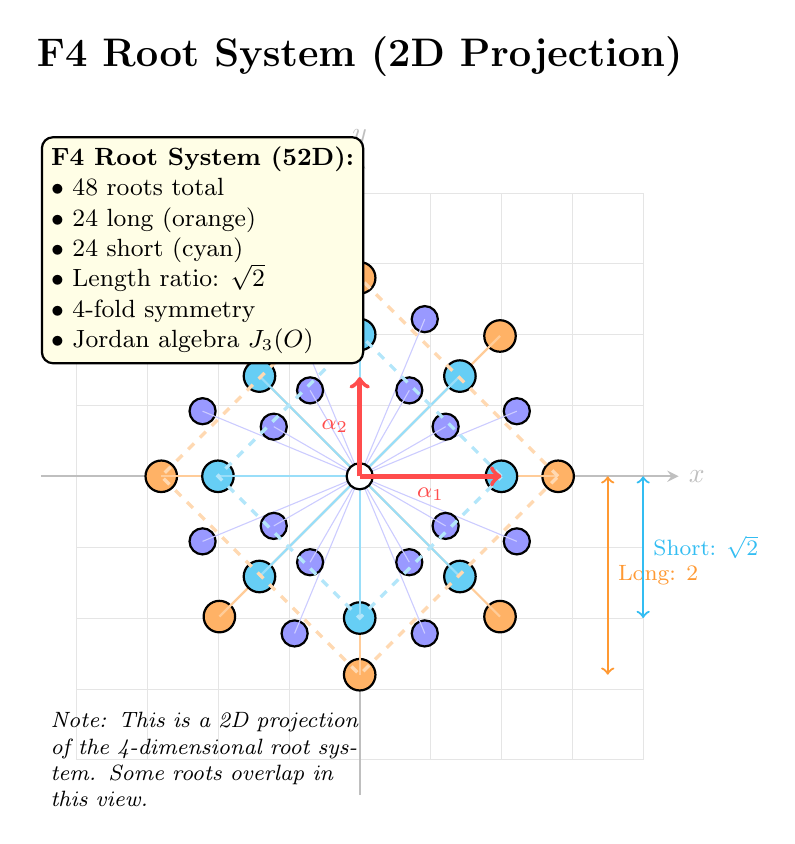
\begin{tikzpicture}[
    scale=0.9,
    root/.style={circle, draw=black, fill=blue!40, thick, minimum size=3mm},
    long_root/.style={circle, draw=black, fill=orange!60, thick, minimum size=4mm},
    short_root/.style={circle, draw=black, fill=cyan!60, thick, minimum size=4mm}
  ]

    % F4 has 48 roots: 24 long, 24 short
    % We project onto a 2D plane showing the characteristic 4-fold symmetry
    % Long roots: length 2, Short roots: length sqrt(2)

    \def\longlen{2.8}
    \def\shortlen{2.0}

    % Draw subtle grid for reference
    \draw[gray!20, very thin] (-4, -4) grid (4, 4);

    % Coordinate axes
    \draw[->, >=stealth, thick, gray!50] (-4.5, 0) -- (4.5, 0) node[right] {$x$};
    \draw[->, >=stealth, thick, gray!50] (0, -4.5) -- (0, 4.5) node[above] {$y$};

    % Long roots aligned with axes (8 roots: +/-2 in each direction)
    \foreach \angle in {0, 90, 180, 270} {
      \pgfmathsetmacro\x{\longlen * cos(\angle)}
      \pgfmathsetmacro\y{\longlen * sin(\angle)}
      \node[long_root] at (\x, \y) {};
      \draw[orange!40, thick] (0, 0) -- (\x, \y);
    }

    % Long roots at 45-degree angles (8 more roots)
    \foreach \angle in {45, 135, 225, 315} {
      \pgfmathsetmacro\x{\longlen * cos(\angle)}
      \pgfmathsetmacro\y{\longlen * sin(\angle)}
      \node[long_root] at (\x, \y) {};
      \draw[orange!40, thick] (0, 0) -- (\x, \y);
    }

    % Short roots aligned with axes (8 roots)
    \foreach \angle in {0, 90, 180, 270} {
      \pgfmathsetmacro\x{\shortlen * cos(\angle)}
      \pgfmathsetmacro\y{\shortlen * sin(\angle)}
      \node[short_root] at (\x, \y) {};
      \draw[cyan!40, thick] (0, 0) -- (\x, \y);
    }

    % Short roots at 45-degree angles (8 more roots)
    \foreach \angle in {45, 135, 225, 315} {
      \pgfmathsetmacro\x{\shortlen * cos(\angle)}
      \pgfmathsetmacro\y{\shortlen * sin(\angle)}
      \node[short_root] at (\x, \y) {};
      \draw[cyan!40, thick] (0, 0) -- (\x, \y);
    }

    % Additional roots at intermediate positions (partial projection)
    % These represent roots that don't lie perfectly in this 2D plane
    \foreach \angle in {22.5, 67.5, 112.5, 157.5, 202.5, 247.5, 292.5, 337.5} {
      \pgfmathsetmacro\x{2.4 * cos(\angle)}
      \pgfmathsetmacro\y{2.4 * sin(\angle)}
      \node[root] at (\x, \y) {};
      \draw[blue!20, thin] (0, 0) -- (\x, \y);
    }

    % Inner ring of roots (representing 4D projection effects)
    \foreach \angle in {30, 60, 120, 150, 210, 240, 300, 330} {
      \pgfmathsetmacro\x{1.4 * cos(\angle)}
      \pgfmathsetmacro\y{1.4 * sin(\angle)}
      \node[root] at (\x, \y) {};
      \draw[blue!20, thin] (0, 0) -- (\x, \y);
    }

    % Origin
    \node[circle, draw=black, fill=white, thick, minimum size=3mm] at (0, 0) {};

    % Highlight 4-fold symmetry with polygons
    \draw[orange!30, very thick, dashed]
      (\longlen, 0) -- (0, \longlen) -- (-\longlen, 0) -- (0, -\longlen) -- cycle;
    \draw[cyan!30, very thick, dashed]
      (\shortlen, 0) -- (0, \shortlen) -- (-\shortlen, 0) -- (0, -\shortlen) -- cycle;

    % Annotations
    \node[anchor=north west, align=left, font=\small, draw=black, fill=yellow!10, rounded corners, thick]
      at (-4.5, 4.8) {
      \textbf{F4 Root System (52D):} \\
      $\bullet$ 48 roots total \\
      $\bullet$ 24 long (orange) \\
      $\bullet$ 24 short (cyan) \\
      $\bullet$ Length ratio: $\sqrt{2}$ \\
      $\bullet$ 4-fold symmetry \\
      $\bullet$ Jordan algebra $J_3(\mathbb{O})$
    };

    % Simple root indicators
    \draw[->, ultra thick, red!70] (0, 0) -- (2.0, 0) node[midway, below, font=\footnotesize] {$\alpha_1$};
    \draw[->, ultra thick, red!70] (0, 0) -- (0, 1.4) node[midway, left, font=\footnotesize] {$\alpha_2$};

    % Root length scale
    \draw[<->, thick, orange!80] (3.5, -\longlen) -- (3.5, 0)
      node[midway, right, font=\footnotesize] {Long: $2$};
    \draw[<->, thick, cyan!80] (4.0, -\shortlen) -- (4.0, 0)
      node[midway, right, font=\footnotesize] {Short: $\sqrt{2}$};

    % Title
    \node[anchor=south, font=\Large\bfseries] at (0, 5.5) {F4 Root System (2D Projection)};

    % Projection note
    \node[anchor=south west, font=\footnotesize\itshape, text width=4cm, align=left]
      at (-4.5, -4.8) {
      Note: This is a 2D projection of the 4-dimensional root system.
      Some roots overlap in this view.
    };

  \end{tikzpicture}
  \caption{Two-dimensional projection of the F4 exceptional Lie algebra root system (dimension 52).
    The 48 roots consist of 24 long roots (orange, length 2) and 24 short roots (cyan, length
    $\sqrt{2}$), giving a length ratio of $\sqrt{2}$. The projection reveals the characteristic
    4-fold rotational symmetry. F4 is the automorphism group of the exceptional Jordan algebra
    $J_3(\mathbb{O})$ (3$\times$3 octonionic Hermitian matrices), connecting it to quantum mechanics
    via the Jordan formulation. The dashed squares show the symmetry structure. Some roots appear
    overlapped due to projection from 4D to 2D; the full structure exists in higher dimensions.}
  \label{fig:f4-root-projection}
\end{figure}
